\chapter{Customizable Contraction Hierarchies}\label{sec:Preliminary_CCH}

In this section we will present the basic idea of \cite[Customization Contraction Hierarchies]{CCH} and also work out the main difference between CCH and \cite[Contraction Hierarchies]{Geisberger_2012}.
It is far form being complete, but there will be some easy examples to show the concept. 

\section{Contracting and Searching}

\begin{figure}
    \centering
    \input{assets/tikz/contractingAndSeaching.tex}
    \caption{The numbers inside the vertices represent their contraction order}
    \label{fig:contrating_and_searching}
\end{figure}

In Figure \ref{fig:contrating_and_searching} you can see a contracted graph $G(V,E')$. The solid lines represent the original edges $E$ of a graph $G$. The dashed lines between vertices are shortcuts $S$ that 
have been added while creating the CCH index graph G'(V, E'). The numbers inside the vertices reflect the contraction order.
\\
Contracting a vertex means deleting it. While contracting a vertex we want to preserve its via connection. If a vertex that is contracted resides on a simple path between two vertices of higher rank,
and there is no edge $e \epsilon E'$ between these vertices a shortcut has to be inserted between the two. 
Let's reconstruct the contraction of Figure \ref{fig:contrating_and_searching}. At first vertex $v(1)$ is removed. As $v(1)$ resides on a simple path to between $v(3)$ and $v(5)$ and there is no edge $e(v(3), v(5)) \notin E'$,
there must be a shortcut insert to keep the via path.
The same applies after contracting $v(2)$ for the vertices $v(4)$ and $v(5)$. For all the other vertices we do not need to insert shortcuts.
\\
As we preserved all via paths during the contraction the shortest path can be retrieved by a bidirectional Dijkstra that is restricted such that it only expands vertices of higher rank. 
Note that the target side walks the in counter direction. 
Therefore if one wants to retrieve the shortest path between $v(3)$ and $v(4)$ there will be a forward search from $v(3)$ and a backward search from $v(4)$. As we restrict theses searches to expand only vertices
of higher rank, the only vertex to expand is $v(5)$ for both searches which is is a meeting point, too. Finding at least one meeting point in the forward an backward search means there exist a path between them.
After merging these paths at the middle vertex $v(5)$ one will obtain the shortest path.
\\
For an arbitrary contracted graph is it possible that there are more than one meeting point. As merging two shortest paths will not necessary lead to an other shortest path, one has to merge
all possible meeting points and take the path among the merged ones which has the smallest distance. 
\\ 
The stopping condition for such a CH-Search is either, both forward and backward search, have reached the top node so there is no further vertex to expand, which happens in the example of figure \ref{fig:contrating_and_searching} or, backward and forward search exceed to 
the length that has already been found among the merged paths.

\section{Difference between CH and CCH}

Looking at the left graph in Figure \ref*{fig:DifferenceCHAndCCH} it has been contracted in the CH way, whereas the right is the CCH way. We explicitly state this here because 
we have found paper \cite{Ouyang_2020} that mix up these well known names, claiming they to Contraction Hierarchies CH while actually doing Customizable Contraction Hierarchies CCH. 
The main difference is, CH will only insert an shortcut between two nodes if the node that is contracted resides on the shortest path between two of its neighbors. 
When vertex $v(1)$ is contracted there is no shortcut inserted as vertex $v(1)$ is not on the shortest path between which is via vertex $v(4)$.
\\
whereas in the CCH case the edge weights do not play a role a contraction time. If a node is contracted and there is no direct connection between two of its neighbors, one has to insert a shortcut. This gives
the advantage that later on we can easily update edge weights without inserting new shortcut, as all possibly needed shortcuts already exist.
\\ 
Let's complete this example by updating the edge $e(v(2), v(4))$ that currently has the weight of $w(e)=1$ to $w(e) = 5$. Now the vertex $v(1)$ is on the shortest path between vertex $v(2)$ and $v(3)$. 
To update the CH graph we have to insert an edge between vertex $v(2)$ and $v(3)$ whereas the topological structure of the CCH remains the same, one only need to update the weight and the middle node of the already give shortcut.

\begin{figure}
    \centering
    \input{assets/tikz/DifferenceCHAndCCH.tex}
    \caption{The left represents a CH and the right a CCH contracted graph}
    \label{fig:DifferenceCHAndCCH}
\end{figure}

\section{Metric Dependent Vertex Order}
There are two ways to get a suitable vertex order. A so called \textit{metric independent} and a so called \textit{metric dependent} one. The metric independent recursively uses balanced separator to determine a vertex ordering\cite{CCH}. Although this is the superior method, it is not used in this paper writing an algorithm that calculates balanced separators isn't trivial, and we are not aiming for optimizing the contraction process. 
The metric dependent order mainly uses the edge difference $ED$ to determine which vertex is to be contracted next. The $ED$ is determined as the $|edges To Insert| - |edges To Remove|$. The fewer edges are inserted during contraction the fewer edges will be contained by the final graph, therefore fewer edges to expand in a search. However using only the edge differences doesn't lead to desired result. This is because during contraction there will be areas that get less dense than others. 
There are two problems that can arise. One is that important vertices are not contracted last. The other is the search space of the query gets linear although it could be logarithmic.

\subsection{Important Vertices not contracted last}\label{sec:not_contracted_last}

\begin{figure}
    \centering
    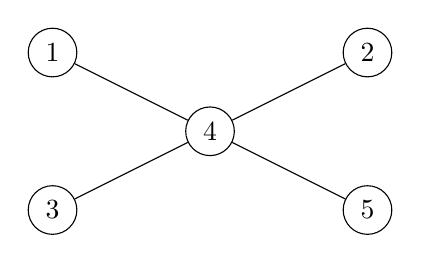
\begin{tikzpicture}[node distance={15mm}, main/.style = {draw, circle}]
    \node[main] (x1) at (1, 2) {$1$}; 
    \node[main] (x3) at (1, 0) {$3$};
    
    \node[main] (x4) at (3, 1) {$4$}; 
    
    \node[main] (x2) at (5, 2) {$2$}; 
    \node[main] (x5) at (5, 0) {$5$}; 
    
    \draw (x1) -- (x4);
    \draw (x2) -- (x4);
    \draw (x3) -- (x4);
    \draw (x5) -- (x4);
    
\end{tikzpicture} 
    
    \caption{The numbers inside the vertices represent their contraction order}
    \label{fig:not_contracted_last}
\end{figure}

Looking at figure \ref{fig:not_contracted_last}, this is a possible contraction order, if only the $ED$ is used to contract vertices. At the beginning the nodes with rank 1, 2, 3, 5 have the same edge difference, which is $ED = -1$. One edge after another will be removed after contraction and the is no shortcut inserted. This happens until there are only the vertices 4 and 5 left. Now vertex 4 has an $ED=-1$, too, same as vertex 5. Therefore the algorithm contracts the vertex with rank 4 before the one with rank 5. \\
However this is not the desired result. There are six ${(1,2), (1,3), (1,5), (2,3), (2,5), (3,5)}$ shortest paths that involve vertex 4, all the other vertices do not encode any shortest path, so vertex 4 should be contracted last. The search graph on the right of Figure \ref{fig:not_contracted_last} shows why. Imagine we we do a shortest path query between $v(1)$ and $v(3)$. After expanding both, the forward and the backward search, to $v(4)$ there is yet another vertex we'll have to expand $v(5)$, although 
as you can see in the original graph on the right, its not possible that $v(5)$ is on the shortest path. Therefore a better contraction order would be a in Figure \ref{fig:contrating_and_searching}.  This can be overcome by the method that is explained in section \ref{sec:vertex_importance}.

\subsection{Linear Query Search Space}\label{sec:linear_query}

\begin{figure}
\centering
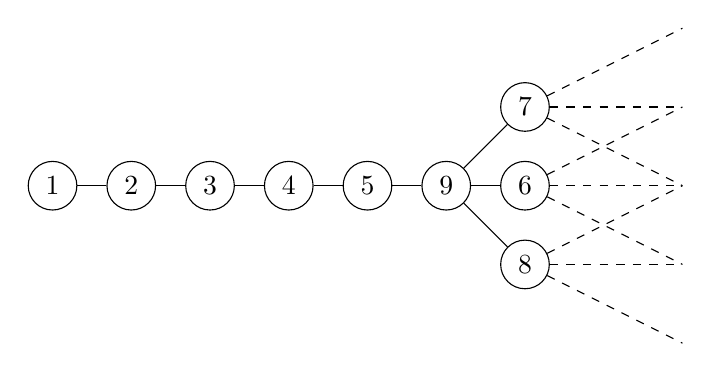
\begin{tikzpicture}[node distance={15mm}, main/.style = {draw, circle}]

    \node[main] (x1) at (0, 0) {$1$};
    \node[main] (x2) at (1, 0) {$2$};
    \node[main] (x3) at (2, 0) {$3$};
    \node[main] (x4) at (3, 0) {$4$};
    \node[main] (x5) at (4, 0) {$5$};
    \node[main] (x9) at (5, 0) {$9$};
    
    \node[main] (x7) at (6, 1) {$7$};
    \node[main] (x8) at (6, -1) {$8$};
    \node[main] (x6) at (6, 0) {$6$};
    
    
    \draw (x1) -- (x2);
    \draw (x2) -- (x3);
    \draw (x3) -- (x4);
    \draw (x4) -- (x5);
    \draw (x5) -- (x9);
    
    \draw (x6) -- (x9);
    \draw (x9) -- (x7);
    \draw (x9) -- (x8);
    
    \draw [dashed] (x7) -- (8, 2);
    \draw [dashed] (x7) -- (8, 1);
    \draw [dashed] (x7) -- (8, 0);
    
    \draw [dashed] (x8) -- (8, 0);
    \draw [dashed] (x8) -- (8, -2);
    \draw [dashed] (x8) -- (8, -1);
    
    \draw [dashed] (x6) -- (8, 1);
    \draw [dashed] (x6) -- (8, 0);
    \draw [dashed] (x6) -- (8, -1);
    
\end{tikzpicture} 
    
\caption{Linear Contraction}
\label{fig:linear_contraction}
\end{figure}

Regarding figure \ref{fig:linear_contraction} there are three possible index graphs $G'$ of one and the same base graph $G$. The numbers inside the vertices represent the contraction order.
\\
The first one could be contracted using the edge difference $ED$, as always one of the outer vertices with $ED=-1$ was contracted. On the one hand it reaches the optimum in case for textit{least shortcuts inserted}. On the other though it has the worst search space among the three vertex orderings. 
To get from node $v(1)$ to $v(5)$ we have to expand four vertices. 
\\
The second $G'$ one contracts the middle vertices, which encodes the most shortest paths, first and therefore inserts three shortcuts. Although this example has a lot of shortcuts, there are still a lot of vertices to expand in some cases. In case every node of $G$ has a weight of $1$, and one wants to go from $v(1)$ to $v(5)$ the forward search will have to expand four nodes as in the upper first example.
\\
The third example contracts the middle node last. At first it contracts the nodes right next to the middle node. Therefore we have to insert shortcuts between $e(v(3)v(5))$ and $e(v(4), v(5))$.
Therefore no matter what source, target pair we are trying to find in this example, the forward and the backward search will have to expand at most one single node. This example additionally shows that
recursively finding a balanced separator, as proposed in \cite[Customization Contraction Hierarchies]{CCH}, is very a promising method to obtain a good contraction order. Sadly there was no time to 
investigate any further in this direction.  

\section{Vertex importance}\label{sec:vertex_importance}

As shown in section \ref{sec:not_contracted_last} and \ref{sec:linear_query} using only the $ED$ as a metric to determine which vertex to contract next is not sufficient to get a suitable

\section{Perfect Customization}

\begin{figure}
    \centering
    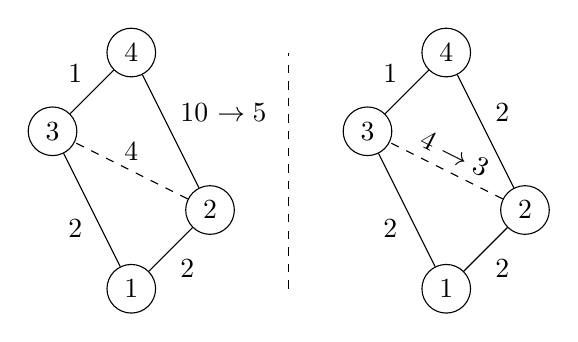
\begin{tikzpicture}[node distance={15mm}, main/.style = {draw, circle}]

    \node[main] (x3) at (0, 2) {$3$};
    \node[main] (x4) at (1, 3) {$4$};
    \node[main] (x2) at (2, 1) {$2$};
    \node[main] (x1) at (1, 0) {$1$};
    
    \draw (x1) -- node[below right] {$2$}(x2);
    \draw (x1) -- node[below left] {$2$} (x3);
    \draw (x2) -- node[above right] {\sout{$10$} $\rightarrow 5$} (x4);
    \draw (x3) -- node[above left] {$1$} (x4);
    \draw[dashed] (x2) -- node[above] {$4$} (x3);

    \draw[dashed]  (3,0) -- (3,3);

    \node[main] (x31) at (4, 2) {$3$};
    \node[main] (x41) at (5, 3) {$4$};
    \node[main] (x21) at (6, 1) {$2$};
    \node[main] (x11) at (5, 0) {$1$};
    
    \draw (x11) -- node[below right] {$2$}(x21);
    \draw (x11) -- node[below left] {$2$} (x31);
    \draw (x21) -- node[above right] {$2$} (x41);
    \draw (x31) -- node[above left] {$1$} (x41);
    \draw[dashed] (x21) -- node[above, sloped] {\sout{$4$} $\rightarrow 3$}  (x31);

    
\end{tikzpicture}
    \caption{Disk Block}
    \label{fig:perfectCustomization}
\end{figure}

Here is an example why perfect customization is necessary to get the full
benefit of CCH.
